\chapter{Week 2: Sept. 18 - 24}
\label{week:2}
\begin{itemize}
    \item Team met with and signed Alex Wong as our supervisor
    \item Back and forth with Lyrical Security about details of NDA and IP agreement
    \item Finished team and advisor contracts
    \item Talked with Alex Wong regarding the details of the NDA
\end{itemize}
    
    \section{Sept 23: Speed Dating Round 1}\label{speed-dating-1}
    \subsection{Team 7: Snow Removal}
    \begin{itemize}
    		\item No good fully automated way
    		\item Risk of injury while removing snow
    		\item Need more affordable options
    		\item Has a good mix of skills in the team members to pull it off
    \end{itemize}
    
    \subsection{Team 10: International Shipping}
    		\begin{itemize}
    			\item Using US + Mexico border as example
    			\item lost of illicit goods being shipped
    			\item Not sure how to tackle it yet
    			\item Looking into modelling the physical steps in shipping and then find ways to improve it.
    			\item One idea is a tamper proof seal
    		\end{itemize}
    		
    \subsection{Team 5: Heat Exhaustion}
    \begin{itemize}
    		\item Early detection of heat exhaustions
    		\item \#2 cause of death for athletes in US
    		\item Health damage or death can happen from heat exhaustion
    		\item Need to measure a good approximation of internal body temp to be able to detect it
    		\item Prof Stashuk as advisor. Good choice
    \end{itemize}
    
        \subsection{Team 1: Real Time Wait Time}
    \begin{itemize}
    		\item How busy is the restaurant I want to go to?
    		\item How long will be the wait time?
    		\item One challenge is to take into consideration crowds inside and outside the location
    		\item Potential for ML
    \end{itemize}
    
        \subsection{Team 2: Women's Health}
    \begin{itemize}
    		\item Uncomfortable topic to talk about
    		\item Lot of stigma
    		\item Chat bot to make this conversation easier
    		\item Source info and knowledge from doctors
    		\item Need to scrape existing forums etc to train the NLP model. This will be challenging
    		\item Should not use conversations to train the model since can lead to mis-training and ruin the purpose - example Microsoft bot
    \end{itemize}
    
        \subsection{Team 4: Pressure Ulcers}
    \begin{itemize}
    		\item Why does it happen?
    		\item How do you prevent it?
    		\item How do you take proactive action towards it?
    \end{itemize}
    
        \subsection{Team 8: Understand Products}
    \begin{itemize}
    		\item Understand existing info about products by using forums, social media reviews etc
    		\item structure this unstructured data somehow - NLP problem
    \end{itemize}
    
    \subsection{Feedback for Us}
    \begin{itemize}
    		\item Try and narrow the scope
    		\item Cannot process each packet in realtime without adding overhead
    		\item Have very clear ways of testing and validating it
    		\item Look at Cloudflare. Potentially have a contact there through someone in class
    \end{itemize}
    
    \section{Tensorflow Example}
    \begin{itemize}
    		\item Started work on a tensorflow example to learn details about neural nets
    \end{itemize}
    
    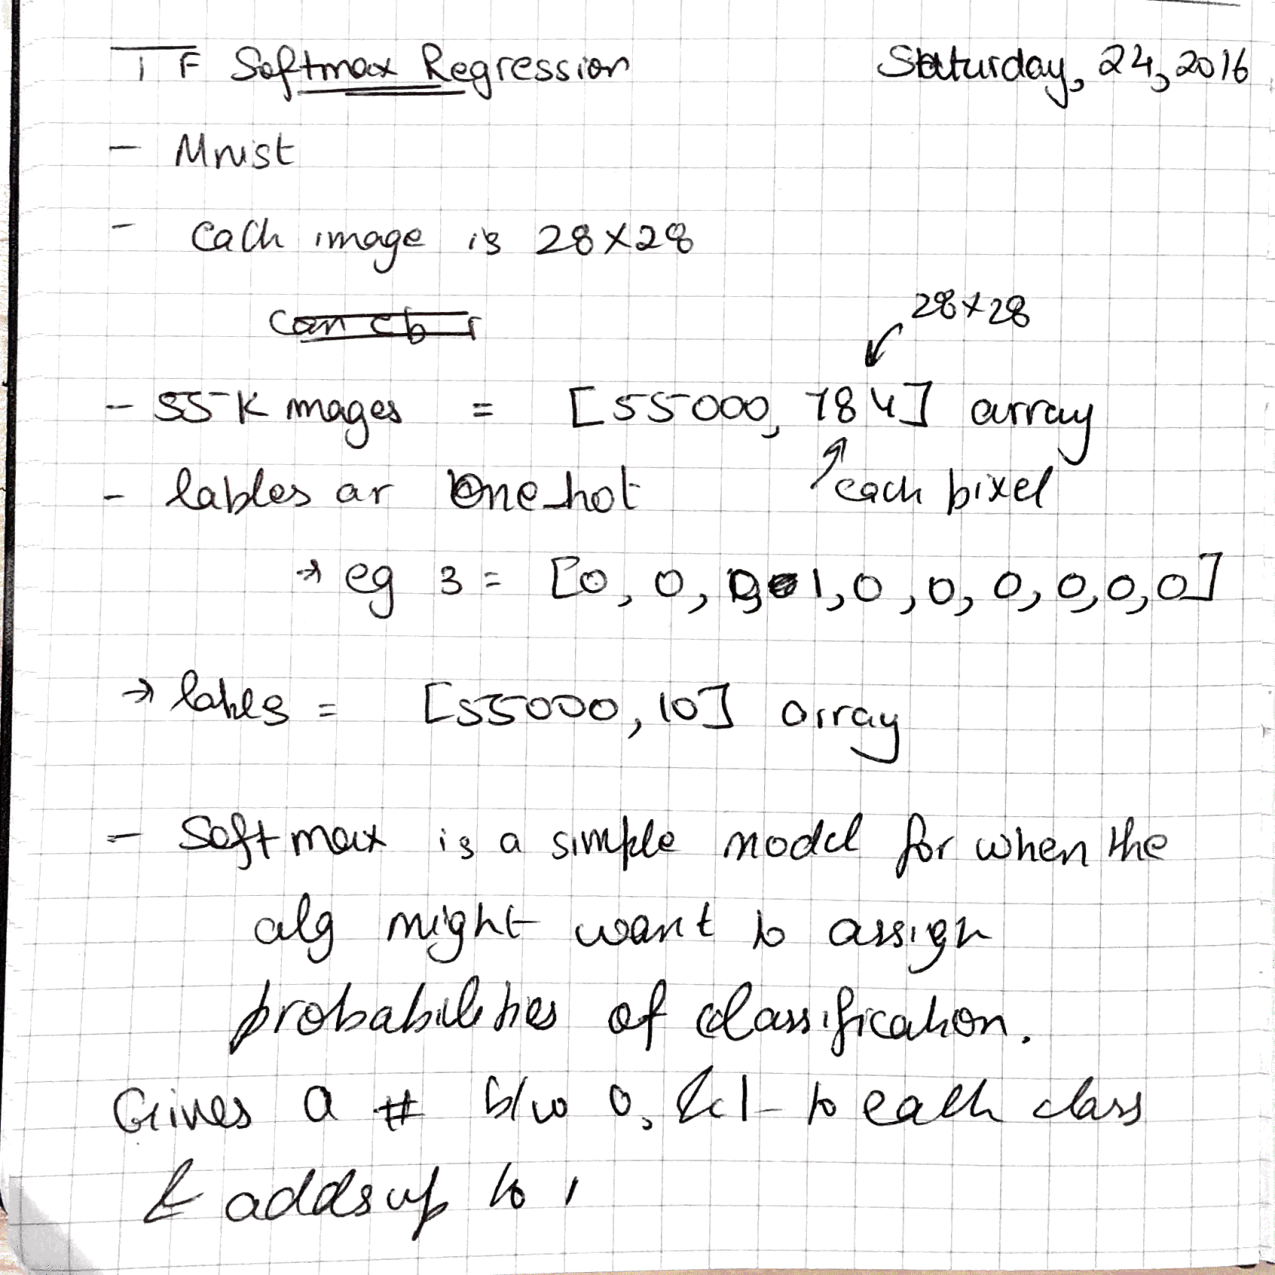
\includepdf[scale=0.7,pages=1]{../pdfs/Sept24-MNIST.pdf}
    \includepdf[scale=1,pages=2]{../pdfs/Sept24-MNIST.pdf}